\documentclass[
	10pt,				    % Schriftgröße
	a4paper,         		% Papierformat
	twocolumn,
	]{article}


\usepackage[T1]{fontenc}
\usepackage{pslatex}
%\usepackage{natbib}
\usepackage[english]{babel}
\usepackage[utf8]{inputenc}
\usepackage[font={footnotesize}]{subcaption}
\usepackage[pdftex]{graphicx}
\usepackage{amsmath}
\usepackage{amssymb}
\usepackage{color, colortbl}
\usepackage{titling}
\usepackage{balance}
\usepackage[letterpaper, inner=1.2cm,top=1.3cm,bottom=2.5cm, textheight=24.0cm,textwidth=19.19cm]{geometry}
\setlength{\columnsep}{0.89cm}
\usepackage{cleveref}
\usepackage{appendix}

\captionsetup{labelfont={normalsize},textfont={normalsize}}
\captionsetup[subfigure]{labelfont={normalsize},textfont={normalsize}}

\captionsetup[table]{labelfont={normalsize}, textfont={normalsize}, labelsep=period}

\usepackage{fancyhdr}
\pagestyle{fancy}

\usepackage{titlesec}

%UNITS
\usepackage[]{units} %writing units

%GRAPHICS
\graphicspath{{Report/Figures}} %path for figures
\usepackage{wrapfig} %wrap text around figures

%BIBLIOGHRAPHY & CITATION
\usepackage[backend=biber,style=numeric,citestyle=numeric,sorting=none]{biblatex}
\addbibresource{references.bib}
\usepackage{csquotes}

\titleformat*{\section}{\filright\normalsize\rmfamily\uppercase}
\titleformat*{\subsection}{\large\bfseries}
%\titleformat*{\subsubsection}{\large\bfseries\itshape}
\titleformat*{\subsection}{\normalsize\rmfamily\bfseries}
%\titleformat{\subsubsection}[block]{\hspace{1em}\small\rmfamily}


\title{\Large \bf
Modelica project - Group 36}

\date{}

\preauthor{}
\DeclareRobustCommand{\authorthing}{
\begin{center}
\begin{tabular}{c c}
\textit{Sindre Hansen} & \textit{Carita Gyldenskog Ranvik}  \\ 
& \\ % Blank row
\textit{Ivan Soløst} & \textit{Thomas Sundvoll}  \\ 
\end{tabular}
\end{center}}
\author{\authorthing}
\postauthor{}


\begin{document}
%\newtheorem{theorem}{Theorem}
\renewcommand\figurename{Fig.}

%\begin{titlingpage}
\setlength{\droptitle}{1.0cm}
\maketitle
\thispagestyle{empty}
\pagestyle{empty}
%\end{titlingpage}
%\thispagestyle{empty}
%\pagestyle{empty}

%\normalsize


\textbf{\textit{Abstract} -- A short abstract (50 to 100 words) in a single paragraph should be included: Tell new or key findings and how you did this study.}
\section*{Abbreviations}

\begin{center}
    \begin{tabular}{l l}
        AE   & Aeration Energy \\
        ASM1 & Activated Sludge Model \\
        BSM1 & Benchmark Simulation Model no. 1 \\
        EQ   & Effluent Quality \\
        IQ   & Influent Quality \\
        ME   & Mixing Energy \\
        PE   & Pump Energy \\
        SP   & Sludge Production
    \end{tabular}
\end{center}

%
%%%%%%%%%%%%%%%%%%%%%%%%%%%%%%%%%%%%%%%%%%%%%%%%%%%%%%%%%%%%%%%%%%%%%%%%%%%%%%%%
\section*{Introduction}\label{sec:Introduction} 
The body of the paper begins with the Introduction. In the introduction you should give a brief overview over Waste Water treatment, answer some questions, for example: What is the main process described by the activated sludge model 1? Why do you need an aerobic and an anaerobic tank? What happens in the aerobic tank and what in the anaerobic (anoxic) tank? What kind of substances do you find in the activated sludge model 1? What does an X indicate and what does and S indicated in the description of the components? What is ammonium? What is denitrification? What is nitrification? The maximal length of the INTRODUCTION is one page.
%
\section{Methods and Theory}\label{sec:METHODS}
%In this section you may want to elaborate a little bit about the theory and methods you used during the project. This can be for instance controller tunings or the relative gain array. \\
%\indent This section should only focus on the methods and theory. It should not contain any results from the project. The maximal length of the METHODS AND THEORY section is one page. 

\subsection{Theory}
\subsubsection{Wastewater quality indicators}
Wastewater quality indicators are test methodologies to assess suitability of wastewater for disposal or re-use, \cite{qi}.

\subsection{Method}
The waste-water treatment plant is modelled and simulated in Dymola using the component-oriented Modelica language. An example model called Activated Sludge Model 1 (ASM1) from a pre-existing waste-water library is used as basis for the model components and composition. The model equations and parameters are implemented based on the Benchmark Simulation Model no. 1 (BSM1) described in \cite{alex2008}. The ASM1 is modified step wise from the default implementation to the implementation representing the BSM1. Simulations are conducted after each step.

Details for each step, including equation and parameter implementation, are described in the following sections.
%
\section*{Assignment 1}\label{sec:Ass1}
%This assignment was about downloading and familiarize ourselves with the wastewater treatment package
The ASM1 BenchPlant example in WasteWater treatment package for Dymola by Gerald Reichl, \cite{wastwater}, was downloaded and simulated with initial values found in \cref{sec: appendB}. By use of ASM1 a simulation model for BSM1 open loop was made by implementation of the following adjustments:\newline
\begin{itemize}
    \item Feedback controllers deleted
    \item Stoichiometry parameters changed to match those in Table 3 of BSM1 report, \cite{alex2008}.
    \item Aeration equation in aeartion tanks "nitri" where set to 
    \begin{equation}
        aeration=kla(So_{sat}-So)
    \end{equation}
    Where the saturation concentration for oxygen is $So_{sat}=8gm^{-3}$. As given in section 2.3.2 of BSM1 report.
    \item Volume and Kla values changed to mach those given in section 2.3.1 and 4 of BSM1 report.
    \item Pump flowrates, $Q_{a}$ and $Q_{w}$, altered to mach those in section 2.1 and 4. $Q_{r}$ set to 18446$m^3d^-1$, given in project description.   
    \item Blower deleted
    \item Temperature inputs deleted
\end{itemize}
A figure of BSM1 Open-loop Dymola Implementation can be found in \cref{fig:openloop}. The open loop configuration has constant source and pump inputs, the system shall therefore reach steady state after some time, as can be seen i our results at this stage. 
%
\section*{Assignment 2 (Dynamic Open-Loop Simulations)}\label{sec:Assignment2}
In this section the system is simulated without controllers and disregarding process noise to verify the model implementation. In each following subsection changes are made step-wise in the model following the specifications in BSM1. Several simulations are conducted with similar initial conditions based on steady-state values from an initial 100-day simulation. For this open-loop assessment the default case control variables, given in section 4 of BSM1, have the constant values $Q_a = \unit[55,338]{m^3/d}$ and $K_La(5) = \unit[84]{d^{-1}}$ (tank 5).

\subsection*{(a)}
Firstly the open-loop system is simulated for 100 days to reach steady state. To do this the waste water source parameters are set as constant, using values from section 3 of BSM1 which are summarized in Table \ref{tab:load-averages}, appendix \ref{sec:AppendixB}. The initial conditions applied to the simulation are given in appendix \ref{sec:AppendixC}, but any arbitrary conditions can be used since the system will reach the same steady-state values with a sufficiently long simulation period.

From the 100-day simulation it can be seen that the state variables of the system stabilizes. To further verify the model selected results at the end of the simulation period, i.e. at steady state, are compared to the corresponding data provided by the project supervisor (mainly based on steady-state results from sections 4 and 5 of BSM1). The comparison is shown in Table \ref{tab:steady-state-results}, appendix \ref{sec:AppendixB}. It is seen that the data coincides down to the last significant digit, which verifies that the open-loop model is implemented correctly. The results are stored in a separate .mat-file so the steady-state values can be used as initial conditions for later simulations. %%%%% USE IN CONCLUSION %%%%% 

\subsection*{(b)}
The next step is to simulate the open-loop system for a 14-day period using provided weather data for the influent parameters. The steady-state values from the previous simulation are used as initial conditions. 

\subsection*{(c)}
In this step a duplicate model is created, but with slight modifications. The system in tank 5 is changed so that the oxygen transfer coefficient gives a constant concentration of dissolved oxygen of $SO = \unit[2]{g/m^3}$. This means that $K_La$ is no longer constant, but vary to output the correct $SO$ instead. The modified system is simulated over 14 days, still using the dry weather data and steady-state initial values from the previous steps. The resulting $K_La$ in tank 5 is shown in figure \ref{fig:KlaTank5}, appendix \ref{sec:AppendixA}. It is clear that $K_La$ is no longer constant

\subsection*{(d)}
\textit{To gauge the performance of the wastewater treatment plant several performance indices have
been proposed in literature. Implement the following performance indices given in section 6
to be calculated by Dymola: EQ, PE, AE, IQ and SP to be calculated over the full time period
from the first day to the 14th day.}

To gauge the performance of the WW treatment plant the following performance indices where implemented: EQ, PE, AE, IQ and SP. The equations related to the WW system performance, EQ, PE, AE, IQ and SP, are defined in Section 6 of the BSM 1 report. The values of $B_i$ in the EQ equation are found in table 10 of the report.  

\textbf{NOTE:} I ligning for $S_NKj0$ bruker vi Xba i stedet for Xxa 

%
\section*{Assignment 3}\label{sec:Ass1}
$\dots$
%
%\section*{Assignment 4}\label{sec:Ass1}
$\dots$
%
\section*{Conclusion}
A brief summary of your results should be included in this section toward the end of the paper.
%
%
\onecolumn
\newpage
\appendix
\begin{appendices}
\section{Figures}
\begin{figure}[htp]
    \centering
    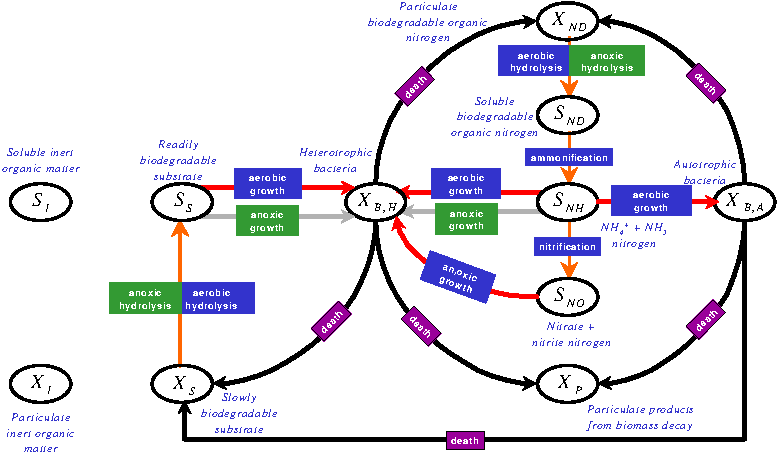
\includegraphics[width=0.6\textwidth]{Report/Figures/asm1-overview.pdf}
    \caption{General overview of ASM1}
    \label{fig:ASM1-overview}
\end{figure}

\newpage

\begin{figure}
    \centering
    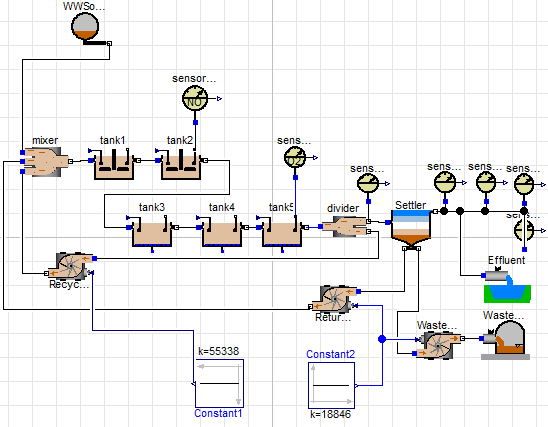
\includegraphics{Report/Figures/task1c.png}
    \caption{BSM1 Open-loop Dymola Implementation}
    \label{fig:openloop}
\end{figure}
\section{Tables}
\newpage
\twocolumn
\section{Initial Values Bench Plant}
\label{sec:AppendixB}
experiment Tolerance=1E-7\\
Settler.S1.X = 6.424263681363e+03\\
Settler.S1.Si = 3.000000000000e+01\\
Settler.S1.Ss = 1.295030132149e+00\\
Settler.S1.So = 1.999998370446e+00\\
Settler.S1.Sno = 1.623473547370e+01\\
Settler.S1.Snh = 2.356727799827e+00\\
Settler.S1.Snd = 5.097661184448e-01\\
Settler.S1.Salk = 3.833472190060e+00\\
Settler.S2.X = 3.858534185097e+02\\
Settler.S2.Si = 3.000000000000e+01\\
Settler.S2.Ss = 1.313469109476e+00\\
Settler.S2.So = 1.999997808673e+00\\
Settler.S2.Sno = 1.596796727152e+01\\
Settler.S2.Snh = 2.620688498604e+00\\
Settler.S2.Snd = 5.149498956479e-01\\
Settler.S2.Salk = 3.866969541077e+00\\
Settler.S3.X = 3.535368422348e+02\\
Settler.S3.Si = 3.000000000000e+01\\
Settler.S3.Ss = 1.326304062865e+00\\
Settler.S3.So = 1.999998505695e+00\\
Settler.S3.Sno = 1.574321763600e+01\\
Settler.S3.Snh = 3.005628887378e+00\\
Settler.S3.Snd = 5.192334322417e-01\\
Settler.S3.Salk = 3.894456624540e+00\\
Settler.S4.X = 3.658163924836e+02\\
Settler.S4.Si = 3.000000000000e+01\\
Settler.S4.Ss = 1.312069378217e+00\\
Settler.S4.So = 2.000000137779e+00\\
Settler.S4.Sno = 1.572405217982e+01\\
Settler.S4.Snh = 3.311901710677e+00\\
Settler.S4.Snd = 5.158389625268e-01\\
Settler.S4.Salk = 3.893033083113e+00\\
Settler.S5.X = 3.927733554733e+02\\
Settler.S5.Si = 3.000000000000e+01\\
Settler.S5.Ss = 1.269942550715e+00\\
Settler.S5.So = 2.000001082463e+00\\
Settler.S5.Sno = 1.603225585080e+01\\
Settler.S5.Snh = 3.353479657344e+00\\
Settler.S5.Snd = 5.030845728215e-01\\
Settler.S5.Salk = 3.845018683832e+00\\
Settler.S6.X = 3.707094910985e+02\\
Settler.S6.Si = 3.000000000000e+01\\
Settler.S6.Ss = 1.241568688152e+00\\
Settler.S6.So = 1.999999828995e+00\\
Settler.S6.Sno = 1.656542580977e+01\\
Settler.S6.Snh = 3.157645899664e+00\\
Settler.S6.Snd = 4.924690064049e-01\\
Settler.S6.Salk = 3.763667982244e+00\\
Settler.S7.X = 7.377320137134e+01\\
Settler.S7.Si = 3.000000000000e+01\\
Settler.S7.Ss = 1.269543710665e+00\\
Settler.S7.So = 2.000001062187e+00\\
Settler.S7.Sno = 1.603779083408e+01\\
Settler.S7.Snh = 3.350596024011e+00\\
Settler.S7.Snd = 5.029453608766e-01\\
Settler.S7.Salk = 3.844215940355e+00\\
Settler.S8.X = 3.082070988771e+01\\
Settler.S8.Si = 3.000000000000e+01\\
Settler.S8.Ss = 1.311404689710e+00\\
Settler.S8.So = 2.000000119719e+00\\
Settler.S8.Sno = 1.573179778908e+01\\
Settler.S8.Snh = 3.309840625819e+00\\
Settler.S8.Snd = 5.156280775302e-01\\
Settler.S8.Salk = 3.892000582300e+00\\
Settler.S9.X = 1.863693081583e+01\\
Settler.S9.Si = 3.000000000000e+01\\
Settler.S9.Ss = 1.326501630233e+00\\
Settler.S9.So = 1.999998510920e+00\\
Settler.S9.Sno = 1.575300220995e+01\\
Settler.S9.Snh = 3.014297581126e+00\\
Settler.S9.Snd = 5.192990500291e-01\\
Settler.S9.Salk = 3.893271573616e+00\\
Settler.S10.X = 1.275536445419e+01\\
Settler.S10.Si = 3.000000000000e+01\\
Settler.S10.Ss = 1.315923153747e+00\\
Settler.S10.So = 1.999997854492e+00\\
Settler.S10.Sno = 1.597856572461e+01\\
Settler.S10.Snh = 2.659914027399e+00\\
Settler.S10.Snd = 5.157153781401e-01\\
Settler.S10.Salk = 3.865860459171e+00\\
tank5.Si = 3.000000000000e+01\\
tank5.Ss = 1.263795984345e+00\\
tank5.Xi = 1.123348086405e+03\\
tank5.Xs = 1.185225923915e+01\\
tank5.Xbh = 2.606406877777e+03\\
tank5.Xba = 1.068019744323e+02\\
tank5.Xp = 4.439932752854e+02\\
tank5.So = 1.999997685099e+00\\
tank5.Sno = 1.674245866877e+01\\
tank5.Snh = 3.117292580061e+00\\
tank5.Snd = 4.979610348992e-01\\
tank5.Xnd = 9.817952441673e-01\\
tank5.Salk = 3.735179685088e+00\\
tank4.Si = 3.000000000000e+01\\
tank4.Ss = 1.965671861503e+00\\
tank4.Xi = 1.119243168969e+03\\
tank4.Xs = 1.995691428575e+01\\
tank4.Xbh = 2.602154360121e+03\\
tank4.Xba = 1.057038911944e+02\\
tank4.Xp = 4.404846296373e+02\\
tank4.So = 3.505091698746e+00\\
tank4.Sno = 1.223560863789e+01\\
tank4.Snh = 7.372095764081e+00\\
tank4.Snd = 6.723187178583e-01\\
tank4.Xnd = 1.509911199178e+00\\
tank4.Salk = 4.336906375072e+00\\
tank3.Si = 3.000000000000e+01\\
tank3.Ss = 3.303021229952e+00\\
tank3.Xi = 1.115644789581e+03\\
tank3.Xs = 4.595646450845e+01\\
tank3.Xbh = 2.587816054472e+03\\
tank3.Xba = 1.042607977985e+02\\
tank3.Xp = 4.368395184843e+02\\
tank3.So = 2.258220736507e+00\\
tank3.Sno = 6.086417053368e+00\\
tank3.Snh = 1.320662231965e+01\\
tank3.Snd = 8.483247444772e-01\\
tank3.Xnd = 3.147367816870e+00\\
tank3.Salk = 5.185981698738e+00\\
tank2.Si = 3.000000000000e+01\\
tank2.Ss = 2.963119860782e+00\\
tank2.Xi = 1.115525591261e+03\\
tank2.Xs = 1.047623215724e+02\\
tank2.Xbh = 2.560547745833e+03\\
tank2.Xba = 1.031268208361e+02\\
tank2.Xp = 4.344353591719e+02\\
tank2.So = 3.460669280848e-05\\
tank2.Sno = 2.374326657217e-01\\
tank2.Snh = 1.943283861745e+01\\
tank2.Snd = 3.395010672094e-01\\
tank2.Xnd = 6.666141082522e+00\\
tank2.Salk = 6.077331022060e+00\\
tank1.Si = 3.000000000000e+01\\
tank1.Ss = 5.744300865020e+00\\
tank1.Xi = 1.114625044801e+03\\
tank1.Xs = 1.056484783737e+02\\
tank1.Xbh = 2.563306641801e+03\\
tank1.Xba = 1.032778829295e+02\\
tank1.Xp = 4.321781192137e+02\\
tank1.So = 4.776381995772e-03\\
tank1.Sno = 1.736044358829e+00\\
tank1.Snh = 1.841130239895e+01\\
tank1.Snd = 1.046350972054e+00\\
tank1.Xnd = 6.244453916847e+00\\
tank1.Salk = 5.956124593796e+00\\

\end{appendices}

\printbibliography

\end{document}